%%%%%%%%%%%%%%%%%%%%%%%%%%%%%%%%%%%%%%%%%%%%%%%%%%%%%%%%%%
%
% Doctoral Thesis Template @ The University of Manchester
% LaTeX Chapter Template
% Version 1 (23/07/2020)
% Joe Crone
%
% This template is based on:
% The University of Manchester, Presentation of Thesis Policy
% Research Office Graduate Education Team
% June 2017
% http://www.regulations.manchester.ac.uk/pgr-presentation-theses/
%
%%%%%%%%%%%%%%%%%%%%%%%%%%%%%%%%%%%%%%%%%%%%%%%%%%%%%%%%%%
\documentclass[../main.tex]{subfiles}
\begin{document}

% Title
%--------------------------------------------------------
\chapter{CBETA Inverse Compton Scattering Source Design}
\label{CBETA_Inverse_Compton_Scattering_Source_Design} % to reference use \ref{ChapterTemplate}

\section{Motivation for a CBETA Inverse Compton Scattering Source}

\section{ERL Electron Beam and Optical Cavity Laser Pulse Parameters}


\begin{table}[!h]
\caption{Electron beam parameters envisaged at the CBETA ICS source interaction point (IP). The given baseline parameters -- which assume the same $\beta^*$ at the IP -- allow a comparison of flux and bandwidth at different energies. The optimised values beneath those are where we have maximised the flux into a 0.5\% scattered photon bandwidth through a suitable combination of beam spot size and collimation angle.}
\vspace{3mm}
\begin{tabular}{lccccc}
\hline\hline
Parameter & \multicolumn{4}{c}{Quantity} & Unit \\
\hline
Turn number & 1 & 2 & 3 & 4 & \\
Electron kinetic energy, $E_e$ & 42 & 78 & 114 & 150 & MeV\\
Repetition rate, $f$ & \multicolumn{4}{c}{162.5} & MHz\\
Bunch charge, $e N_e$ & \multicolumn{4}{c}{32} & pC \\
Transverse normalised \textit{rms} emittance, $\epsilon_{N}$ & \multicolumn{4}{c}{0.3} & mm-mrad\\
\textit{rms} bunch length, $\Delta \tau$ & \multicolumn{4}{c}{1.0 (3.33)} & mm (ps)\\
Relative energy spread & \multicolumn{4}{c}{$5.0\times 10^{-4}$} & \\
\hline
 & \multicolumn{4}{c}{Baseline parameters} & \\
\hline
$\beta^*$ (at the IP) & \multicolumn{4}{c}{1} & cm\\
Electron bunch spot size, $\sigma_{\mathrm{electron}}$ & 6.01 & 4.42 & 3.65 & 3.19  & \si{\micro\meter} \\
\hline
 & \multicolumn{4}{c}{Optimised for 0.5\% bandwidth} & \\
\hline
$\beta^*$ (at the IP) & 3.56 & 6.58 & 9.60 & 12.62 & cm\\
Electron bunch spot size, $\sigma_{\mathrm{electron}}$ & 11.34 & 11.34 & 11.34 & 11.34  & \si{\micro\meter}\\
Collimation angle, $\theta_{\mathrm{col}}$ & 1.533 & 0.830 & 0.569 & 0.433 & mrad\\
\hline\hline
\end{tabular}
\label{TABLE:CBETA_electron_beam_design_parameters}
\end{table}

\begin{table}[!h]
\centering
\caption{Nd:YAG Gaussian laser pulse parameters at the CBETA ICS IP. The laser pulse is produced from a Nd:YAG infrared laser and re-circulated in a bow-tie optical cavity.}
\begin{tabular}{lcc}
\hline\hline
Parameter & Quantity & Unit \\
\hline
Wavelength, $\lambda_\textrm{laser}$ & 1064 & nm\\
Photon energy, $E_\textrm{laser}$ & 1.17 & eV\\
Pulse energy  & 62 & \si{\micro\joule}\\
Number of photons, N_{\textrm{laser}} & $3.3\times 10^{14}$\\ 
Repetition rate, $f$ & 162.5 & MHz\\
Spot size at the IP, $\sigma_\textrm{laser}$ & 25 & \si{\micro\meter}\\
Crossing angle, $\phi$ & 5 & deg \\
Pulse length  & 10 & ps\\
Relative energy spread, $\Delta E_\textrm{laser}/E_\textrm{laser}$ & 6.57$\times 10^{-4}$ &   \\
 % 0.7nm error on 1064nm
\hline\hline
\end{tabular}
\label{TABLE:CBETA_laser_pulse_design_parameters}
\end{table}

\section{Flux - Bandwidth Optimisation}

The bandwidth of an ICS light source is tuneable and can be selected on the basis of user requirements. Here we develop a method to maximise flux within a selected bandwidth for the simplified case of an electron beam with a round transverse profile i.e normalised emittance is identical in both directions ($\epsilon_{nx} = \epsilon_{ny} = \epsilon_{n}$). Bandwidth selection is possible by selecting $\beta^{*}$ at the IP and by setting the collimation angle, $\theta_{\mathrm{col}}$ that collects the scattered photons; these may for example comprise switchable, fixed-aperture collimators.

Within this optimisation derivation, the bandwidth is given by (Eq.~\ref{eq:bandwidth}) with the emittance term (Eq.~\ref{eq:emittance_term}) modified for the transversely round bunch case
\begin{equation}
\frac{\sigma_{\epsilon}}{E_{\epsilon}} = \frac{2\gamma\epsilon_{n}}{\left(1+X\right)\beta^{*}},
\label{eq:emittance_term_round_beam}    
\end{equation}
where $X$ is the recoil parameter (Eq.~\ref{eq:X_geometry}), $\epsilon_{n}$ is the transverse \textit{rms} normalised emittance of the electron bunch and $\beta^{*}$ is the $\beta$-function at the interaction point.

Typically the dominant terms that define the bandwidth of an inverse Compton source Eq.~(\ref{eq:bandwidth}) are the collimation term Eq.~(\ref{eq:collimation_term}) and the emittance term Eq.~(\ref{eq:emittance_term_round_beam}). The free parameter of the collimation term is the collimation angle $\theta_{\mathrm{col}}$, which can be adjusted either by changing the collimator aperture or changing its distance from the IP. Adjustable collimators have been designed for the ELI-NP-GBS $\gamma$-ray ICS source~\cite{paterno2017collimation}; a similar design could be implemented at other ICS sources.

The emittance term is dependent both on the normalised transverse emittance $\epsilon_{n}$ and on $\beta^{*}$. It is more convenient to change the $\beta$-function at the IP with focusing rather than by varying the emittance, since the latter is dependent on the injector and collective effects prior to the IP. By using a larger $\beta^{*}$ and a small collimator aperture, it is possible to reduce the contribution of the collimation and emittance terms so that they are negligible; thus the electron bunch and laser pulse energy spread terms (Eq.~\ref{eq:beam_energy_spread_term},~\ref{eq:laser_energy_spread_term}) become dominant for accelerators with a sufficiently small emittance. This effectively places a lower limit on the bandwidth of an ICS source, i.e. it is limited by the energy spread of the electron beam $\Delta E_{e}/E_{e}$ and laser pulse $\Delta E_{\mathrm{laser}}/E_{\mathrm{laser}}$ as 
\begin{equation}
\left(\frac{\Delta E_{\gamma}}{E_{\gamma}}\right)_{\mathrm{min}} \approx 2 \frac{\Delta E_{e}}{E_{e}} + \frac{\Delta E_{L}}{E_{L}},
\label{eq:bandwidth_limitation_minimum}
\end{equation}
for the low recoil approximation.

Consequently, any bandwidth above this limit can be achieved by an ICS source by tuning of the collimation angle and $\beta^*$ so that a desired bandwidth, $\Delta E_{\gamma}/E_{\gamma}$, is achieved. Since the collimation and emittance terms are typically dominant, all other terms can be excluded and the solutions are bounded by
\begin{equation}
\frac{\Delta E_{\gamma}}{E_{\gamma}} > \sqrt{\left(\frac{ \sigma_{\theta}}{E_{\theta}}\right)^{2}+\left(\frac{\sigma_{\epsilon}}{E_{\epsilon}}\right)^{2}}.    
\end{equation}
This results in myriad combinations of $\beta^{*}$ and $\theta_{\mathrm{col}}$ that satisfy a particular chosen bandwidth larger than this lower limit (Eq.~\ref{eq:bandwidth_limitation_minimum}).

The different $\beta^{*}$, $\theta_{\mathrm{col}}$ combinations each give a different collimated flux; obviously we wish to chose the solution with the largest flux. The collimated flux $\mathcal{F}_{\Psi}$ of each solution is calculated based on a method valid for small collimation angles ($\gamma\theta_{\mathrm{col}} < 1$) derived by Curatolo et al.~\cite{curatolo2017analytical}. Re-cast for our variable definitions, it becomes
\textcolor{blue}{**THIS MAY CHANGE WITH THE NEW COLLIMATED FLUX METHOD**}
% serafini calc
\begin{equation}
\mathcal{F}_{\Psi}\propto \frac{\left(1+\sqrt[3]{X}\Psi^{2}/3\right)\Psi^{2}}{\left[1+\left(1+X/2\right)\Psi^{2}\right]\left(1+\Psi^{2}\right)}, 
\label{eq:curatolo_collimated_flux}
\end{equation}
where $\mathcal{F}$ is the total (uncollimated) flux, $\Psi = \gamma\theta_{\mathrm{col}}$ is the acceptance angle, and $X$ is the recoil parameter. The solution giving the maximal flux is selected.

It is not practicable to calculate the flux from every combination of $\beta^{*}$ and $\theta_{\mathrm{col}}$. Instead, an array of collimation angles $\theta_{\mathrm{col}}$ from 0 to $1/\gamma$ is used ($\gamma\theta_{\mathrm{col}}<1$), and for a given bandwidth value the corresponding $\beta^*$ is calculated using
\begin{equation}
\beta^{*} = \frac{2\gamma\epsilon_{n}}{\left(1+X\right)\sqrt{\left(\frac{\Delta E_{\gamma}}{E_{\gamma}}\right)^{2}-\left[\left(\frac{\sigma_{\theta}}{E_{\theta}}\right)^{2}+\left(\frac{\sigma_{e}}{E_{e}}\right)^{2}+\left(\frac{\sigma_{L}}{E_{L}}\right)^{2}\right]}},
\label{eq:beta_star_round_beam}
\end{equation}
which is a rearrangement of (Eq.~\ref{eq:bandwidth}) with the emittance term in the transversely round bunch case (Eq.~\ref{eq:emittance_term_round_beam}). 

The collimated flux $\mathcal{F}_{\Psi}$ is calculated for each combination produced via this method. The maximal collimated flux is selected and the combination of $\beta^{*}$ and $\theta_{\mathrm{col}}$ corresponding to this solution is returned. This process can be applied to the case of a target bandwidth to determine $\theta_{\mathrm{col}}$, $\beta^{*}$, and collimated flux in the selected bandwidth. In addition, applying this method to a continuum of bandwidths allows us to map the possible operational settings of our ICS source, and to derive tuning curves such as the variation of the collimated flux with bandwidth.

The optimised $\beta^{*}$ and $\theta_{\mathrm{col}}$ of a 0.5\% narrow bandwidth case are shown in Table~\ref{TABLE:CBETA_electron_beam_design_parameters}, with the collimated flux this produces tabulated in Table~\ref{tab:CBETA_spectral_output}. The $\beta^{*}-\theta_{\mathrm{col}}$ parameter space of the CBETA ICS, for all nominal energies, is shown in Fig.~\ref{fig:CBETA_beta_theta_parameter_space}.
\begin{figure}[!h]
\centering
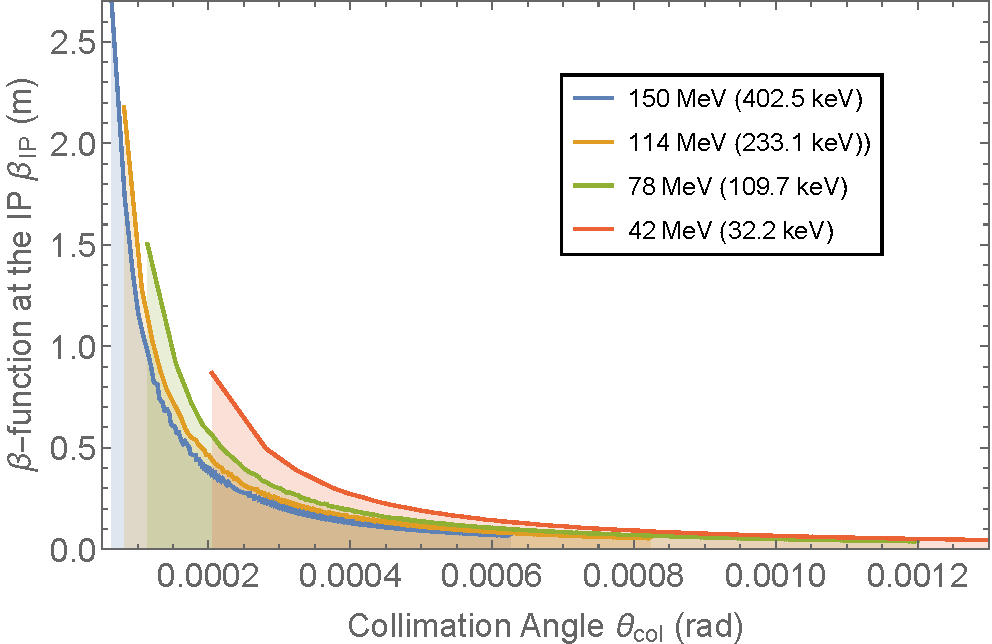
\includegraphics[width=0.7\textwidth]{Figures/CBETA_Inverse_Compton_Source_Design/CBETABetaTheta.pdf}
\caption{Tuning curves of $\beta^{*}$ against $\theta_{\mathrm{col}}$ for each of the nominal CBETA electron beam energies satisfying the maximal flux across the 0--1\% bandwidth range. The shaded area is the parameter space, while the line corresponds to the maximal flux solution for a given bandwidth. Minimised bandwidth solutions in this range have large $\beta$-functions at the IP and small collimation angles $\theta_{\mathrm{col}}$; the maximal bandwidth solutions have small $\beta$-functions and larger collimation angles $\theta_{\mathrm{col}}$.}
\label{fig:CBETA_beta_theta_parameter_space}
\end{figure}

Each of the pareto fronts (for each nominal energy) of the $\beta^{*}-\theta_{\mathrm{col}}$ parameter spaces in Fig.~\ref{fig:CBETA_beta_theta_parameter_space} has a distinctive shape - a linear regime followed by non-linear regime. The pareto front shows a linear relationship as the collimation angle increases, this part is dominated by the emittance term, until a vertex is reached and, as collimation angle increases, there is a non-linear shape, where the pareto front is dominated by the collimation term. The termination of the pareto fronts at the small collimation angle marks the point in which the optimal $\beta$-function at the IP becomes imaginary.

By applying the collimated flux maximisation to the parameter space shown in Fig.~\ref{fig:CBETA_beta_theta_parameter_space}, the collimated flux - bandwidth tuning curve of the CBETA ICS can be discerned, as shown in Fig.~\ref{fig:CBETA_Tuning_Curve}. 
\begin{figure}[!h]
\centering
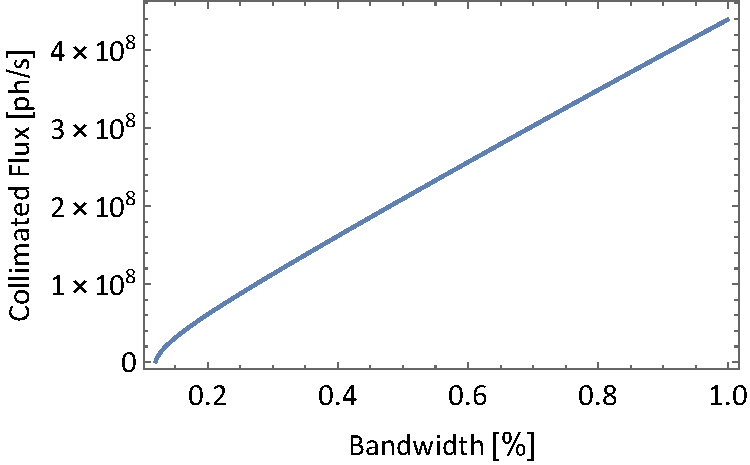
\includegraphics[width=0.7\textwidth]{Figures/CBETA_Inverse_Compton_Source_Design/CBETATuningCurve.pdf}
\caption{Tuning curve of collimated flux against bandwidth for a 0--1\% bandwidth range, produced by tuning $\beta^{*}$ and $\theta_{\mathrm{col}}$. The tuning curve is independent of beam energy for scattering scenarios within the Thomson regime, hence this tuning curve applies to all energies in CBETA. The left end of tuning curve indicates the minimum possible bandwidth of the ICS source, which in CBETA is $\simeq$~0.1\% and is determined by the electron beam energy spread.}
\label{fig:CBETA_Tuning_Curve}
\end{figure}

In Fig.~\ref{fig:CBETA_Tuning_Curve}, the tuning curves of the four nominal energies of the CBETA ICS are shown as a single line. This is as the recoil parameter for the CBETA ICS is near-negligible for the operating energy of CBETA, which means the tuning curves directly overlap. The relationship between collimated flux and bandwidth for the CBETA ICS is linear past the rapid fall off at low bandwidth which is occurs once we approach the minimum theoretical limit of the bandwidth. Within the non-linear range of Fig.~\ref{fig:CBETA_Tuning_Curve} the energy spreads of the electron bunch and laser pulse dominate the bandwidth, which restricts the $\beta^{*}$-$\theta_{\mathrm{col}}$ parameter space. Consequently the optimum balance between the emittance and collimation term can not be achieved, causing a rapid decrease in the collimated flux.   

\section{Bypass Design}

To utilize CBETA as an inverse Compton scattering source at the 150~\si{\mega\electronvolt} maximum electron beam energy, a bypass line is required that replaces the ordinary 4th pass due to the stringent space restrictions in the existing FFA system; this leaves no space to arrange IP focusing, nor for the laser re-circulation cavity. The scattered photons from the ICS must also be produced in a different plane to the existing accelerator; the photons must be safely extracted from the footprint of the ERL since there is no space for an experimental hutch within the existing CBETA hall. This is evident upon inspection of Fig.~\ref{fig:CBETA_schematic} the technical schematic of the CBETA accelerator and hall. From this diagram it is also clear that there is no scope to build a bypass line within the same plane as the existing accelerator due to space constraints.

\begin{figure}[!h]
\centering
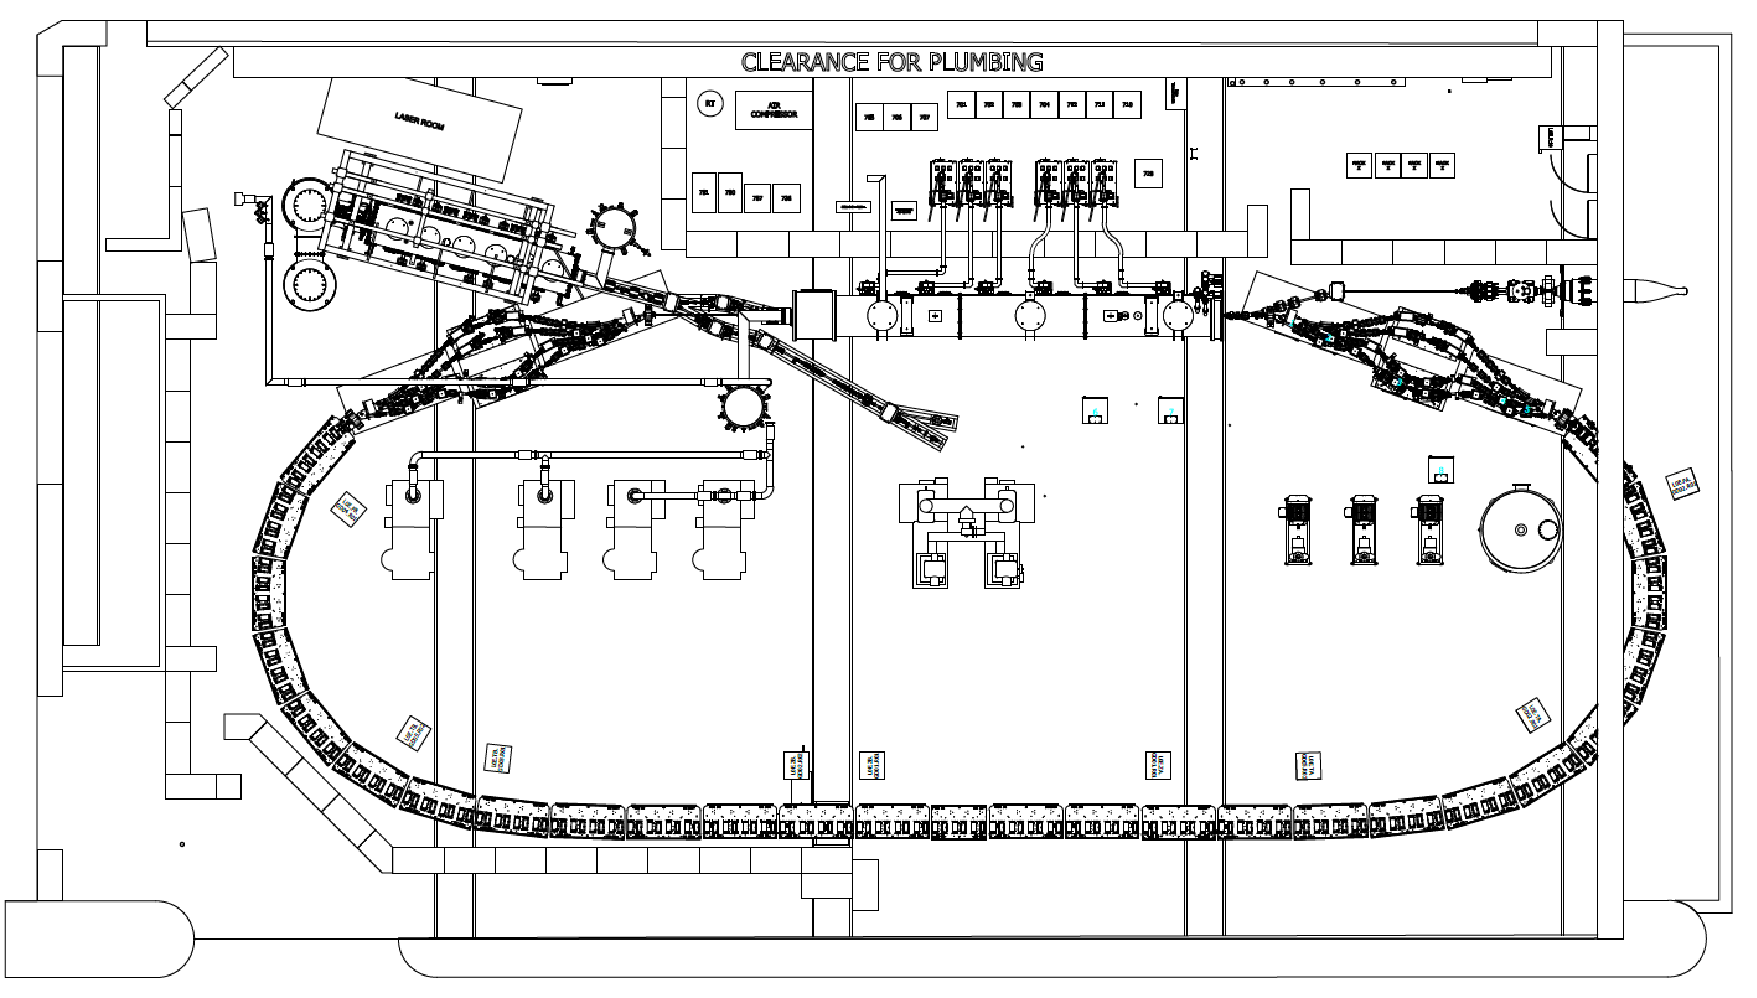
\includegraphics[width=0.8\textwidth]{Figures/CBETA_Inverse_Compton_Source_Design/CBETA_schematic.pdf}
\caption{Schematic of the CBETA ERL; existing accelerator structure including injector, main linac cryomodule, FFAG return loop, splitter and recombiner systems and beam dump, as well as supporting infrastructure such as electronic racks, vaccuum pumps and shielding. \textcolor{blue}{Who do I reference for this? Ask Kirsten!}}
\label{fig:CBETA_schematic}
\end{figure}

The layout of such a bypass line is shown in Fig.~\ref{fig:CBETA_ICS_Layout}. The bypass is configured for 150~\si{\mega\electronvolt} 4th-pass operation but could be adapted to operate with all nominal energies. The bypass was designed and optimised using the \textsc{Bmad} accelerator simulation library~\cite{BmadManual} and the \textsc{Tao} program~\cite{TaoManual} for simulating high
energy particle beams in accelerators.

\begin{figure}[!h]
\centering
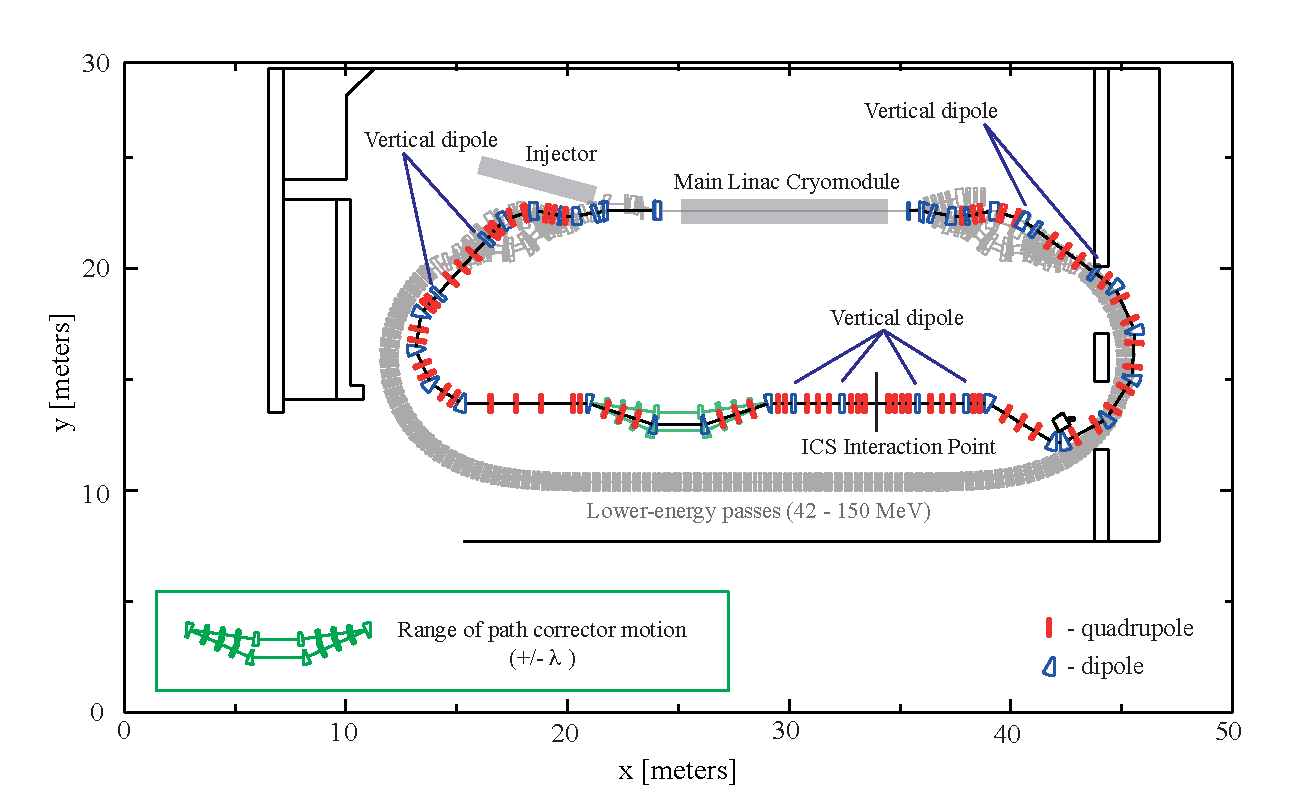
\includegraphics[width=0.8\textwidth]{Figures/CBETA_Inverse_Compton_Source_Design/cbetaicslayout.pdf}
\caption{Layout of the ICS bypass in CBETA; greyed beamline elements are already installed in the existing accelerator. Outer walls and relevant existing infrastructure shown in black.}
\label{fig:CBETA_ICS_Layout}
\end{figure}

The bypass line diverts the 150~\si{\mega\electronvolt} electron beam after the 4th linac pass in the corresponding S4 splitter line; the electron beam then re-enters the existing layout in the R4 line. The bypass replaces the FFA return loop, S4, from the 4th dipole onward and R4 up to the 4th dipole. The bypass will be located above the existing permanent magnet arc as the FFA arc is still used to transport the lower energy (42, 78, and 114~MeV) beams before and after the bypass.

A system of vertical doglegs, replacing sections of the S4 and R4 lines, are required to provide a 30~\si{\centi\meter} vertical elevation of the bypass line relative to the plane of the FFA return loop in order to avoid the existing accelerator. Bypass arc sections replace the existing FFA arc sections (FA, FB). Following the first arc, there is a horizontal dogleg used to close horizontal dispersion before the interaction region and offset the bypass from existing infrastructure. 

At the interaction region (IR) the beam is again offset upward locally by a further 20~\si{\centi\meter} -- to a 50~\si{\centi\meter} total offset above the FFA reference orbit height -- using a pair of vertical doglegs; these are here called the IR doglegs. The further vertical offset is imposed so the photons are produced in a different plane to both the bypass line and FFA return loop which is necessary for the extraction of the x-ray beam to an external experimental hutch and in order to avoid irradiation of the FFA permanent magnets. A flexible focusing section within the pair of IR doglegs is used to focus to the required beam waist. The final focus section is designed to enable both $\beta^{*} = 1$~\si{\centi\meter} for the baseline case and $\beta^{*} = 12.6$~\si{\centi\meter} for the 0.5\% bandwidth case (see Table~\ref{TABLE:CBETA_electron_beam_design_parameters}). The final focus section is constructed from 7 quadrupoles with the laser re-circulation cavity placed between the 4th and 5th quadrupole. This scheme allows the photons to be extracted via the first dipole of the downstream IR dogleg, minimizing the number of magnets requiring modification for photon extraction. 

Within the straight section of the bypass following the IR, a variable path length adjustment is implemented based on the moving chicane described by H. Owen et al~\cite{owen2012modular}; this 4-dipole focusing chicane uses two mechanically-adjustable swing arms each incorporating a quadrupole triplet, and a central bellows. The chicane replicates the function of the S4/R4 splitter/recombiners to allow variation of both $R_{56}$ and path length for re-entry into the MLC. Path length adjustment is made by opening the swing arms whilst increasing the dipole strengths accordingly; over a change in path length of $\pm\lambda_{RF}$ the variation in Twiss values (after re-matching) is moderate.

Optics tuning of the bypass is limited by the compact layout of CBETA, the conditions required for energy recovery of the interacted beam ($R_{56}=0$), and the necessity for the bypass to be constructed above the existing FFA return loop; the $\beta$-functions and dispersion are however still feasible. Plots of $\beta$-functions and dispersion in the bypass line for the 0.5\% bandwidth case are shown in Figs.~\ref{fig:CBETA_ICS_Twiss} and~\ref{fig:CBETA_ICS_dispersion}. 

\begin{figure}[!h]
    \centering
    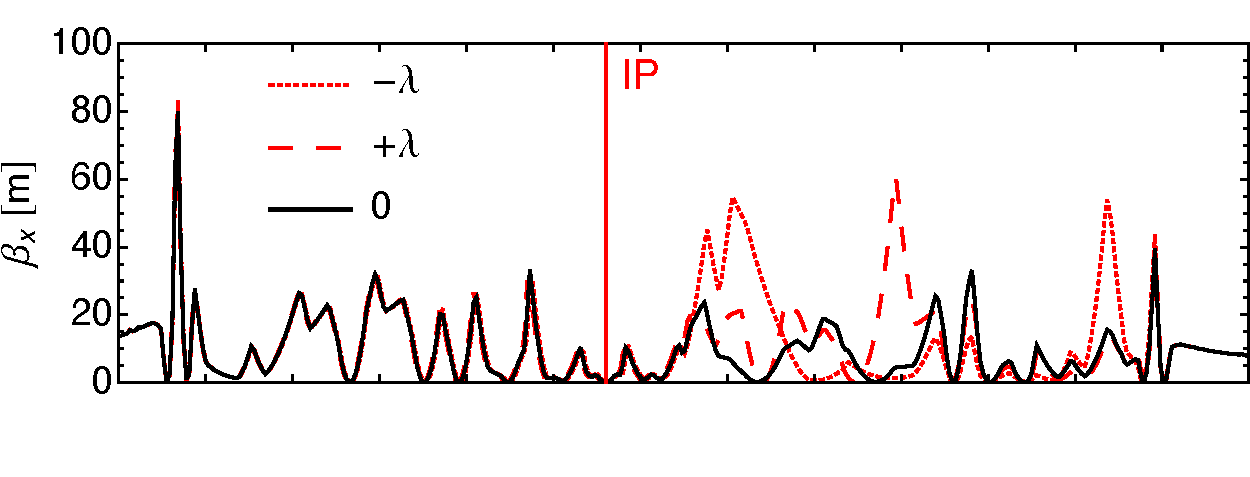
\includegraphics[width=0.5\textwidth]{Figures/CBETA_Inverse_Compton_Source_Design/twissplotx.pdf}
    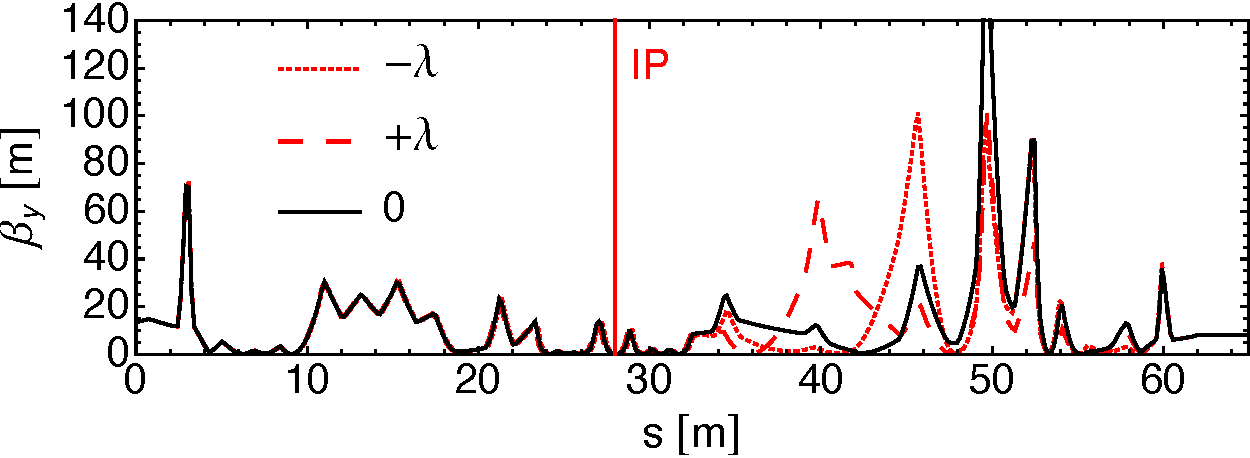
\includegraphics[width=0.5\textwidth]{Figures/CBETA_Inverse_Compton_Source_Design/twissploty.pdf}
    \caption{Twiss functions in the ICS bypass line, showing the re-matched conditions for different path length configurations $-\lambda_{RF}$, $0$ and $+\lambda_{RF}$. The ICS interaction point (IP) is indicated. \textcolor{blue}{Potentially worth putting the beta functions and dispersion functions side by side?}}
    \label{fig:CBETA_ICS_Twiss}
\end{figure}

\begin{figure}[!h]
\centering
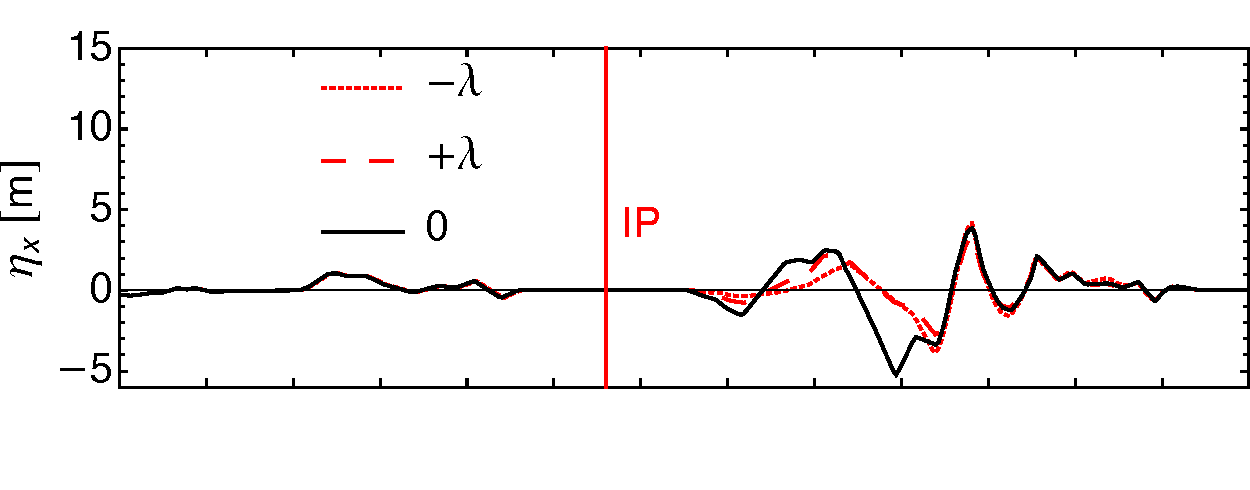
\includegraphics[width=0.5\textwidth]{Figures/CBETA_Inverse_Compton_Source_Design/dispplotx.pdf}
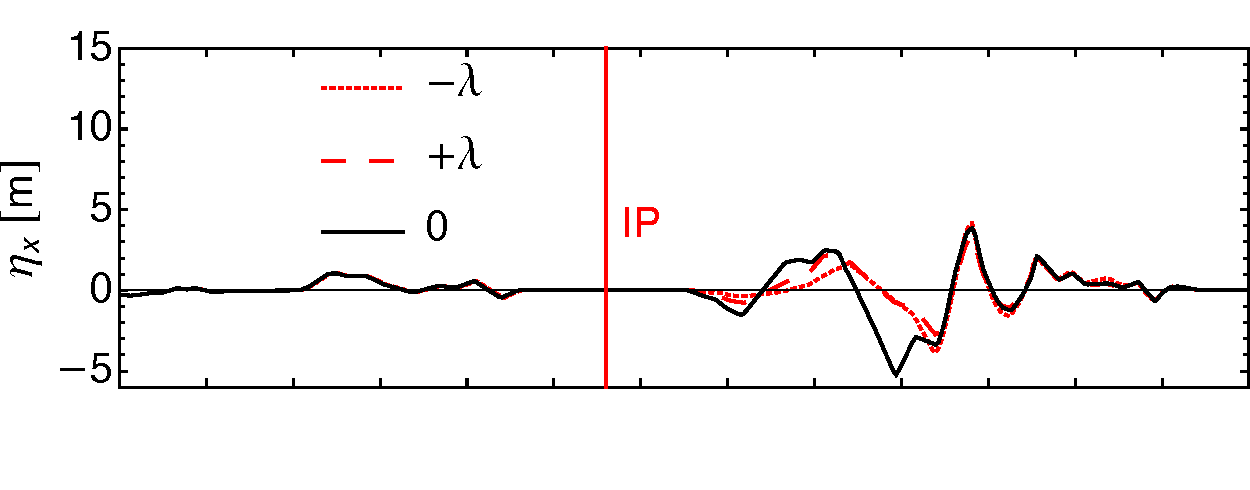
\includegraphics[width=0.5\textwidth]{Figures/CBETA_Inverse_Compton_Source_Design/dispplotx.pdf}
\caption{Dispersion functions in the ICS bypass line for the 0.5\% bandwidth case, showing the re-matched conditions for different path length configurations $-\lambda_{RF}$, $0$ and $+\lambda_{RF}$. The ICS interaction point (IP) is indicated.}
\label{fig:CBETA_ICS_dispersion}
\end{figure}

The solution for the 150~\si{\mega\electronvolt} 4th pass could be generalised to the lower energy passes to form configurable ICS sources from each line. Electron bunches would be re-routed through the S4 line, magnet strengths would be scaled and re-matched, the optimised IP focusing solution for each line, as in Table~\ref{TABLE:CBETA_electron_beam_design_parameters} would be adhered to, and the path length correction system demonstrates the necessary flexibility for $\pm\lambda_{RF}$ adjustment which would be sufficient.

The 150~\si{\mega\electronvolt} nominal energy is potentially the most challenging as this requires the highest gradient magnets for focusing at the IP, path length correction and transport. However, in standard 4-pass operation this transport line is only traversed once, each other line is traversed twice in both acceleration and deceleration configuration.

For example the 3rd pass 114~\si{\mega\electronvolt} nominal energy transport line is traversed on both the 3rd turn (accelerating pass) and the 5th turn (decelerating pass). The result is that if the ERL is still operated in 4-pass mode the bypass line (for the 3rd pass) has to satisfy both sets of conditions imposed on the accelerating and decelerating pass, whilst still achieving the same IP focusing constraints. Alternatively, the ERL could be operated as a 3-pass ERL for the purpose of an ICS at the 3rd nominal energy which would require sufficient flexibility within a bypass ICS line in order to operate as a multi-colour photon source.

The author favours the latter solution to this problem as common transport systems in ERLs are already typically highly constrained - more-so for the FFAG multiple energy common transport system in CBETA  (\textcolor{blue}{reference to the relevant part in CBETA ERL commissioning}) - and the latter solution appears to offer less constraints on the beam dynamics. Of course, this issue could be avoided entirely via the use of single transport, where we have different transport beamlines for both the accelerating and decelerating configuration of each nominal energy of the multi-turn ERL, with ICS interaction points integrated, not retrofitted into the design.     

\section{Spectral Output}

\begin{table}[!h]
\caption{Anticipated photon output for each of the four electron beam energies in CBETA, taking into account a 5~degree crossing angle. The uncollimated flux varies by around 2\% due to the small effect of the electron spot size; $X < 0.003$ even at 150~MeV. The collimated flux has been optimised for a 0.5\% bandwidth. The number of scattered photons is essentially independent of electron energy for a fixed electron spot size at the IP, and since both the Compton spectrum and the (relative) 0.5\% bandwidth scale together with $\gamma^2$, both the optimised spot size and the predicted collimated fluxes are the same at all electron energies.}
\scalebox{0.92}{
\begin{tabular}{lccccc}
\hline\hline
 & \multicolumn{4}{c}{Electron Kinetic Energy (MeV)} & \\
 \cline{2-5}
 & 42 & 78 & 114 & 150 & Unit \\
\hline
X-ray peak energy & 32.2 & 109.7 & 233.1 & 402.5 & keV\\
Source Size & 5.84 & 4.35 & 3.62 & 3.17 & \si{\micro\meter} \\
Uncollimated flux & 3.16$\times10^{10}$ & 3.20$\times10^{10}$ & 3.21$\times10^{10}$ & 3.22$\times10^{10}$ & ph/s\\
Spectral density & 9.82$\times10^{5}$ & 2.92$\times10^{5}$ & 1.38$\times10^{5}$ & 8.00$\times10^{4}$ & ph/s eV\\
Average brilliance & 9.23$\times10^{10}$ & 3.19$\times10^{11}$ & 6.81$\times 10^{11}$ & 1.18$\times10^{12}$ & ph/s mm$^{2}$ mrad$^{2}$ 0.1\% bw\\
Peak brilliance & 2.80$\times 10^{15}$ & 1.00$\times 10^{16}$ & 2.18$\times10^{16}$ & 3.80$\times 10^{16}$ & ph/s mm$^{2}$ mrad$^{2}$ 0.1\% bw\\
\hline
 & \multicolumn{4}{c}{0.5\% bandwidth} & \\
\hline
Source Size & 10.25 & 10.34 & 10.32 & 10.35 & \si{\micro\meter} \\ 
Collimated flux & 2.09$\times 10^{8}$ & 2.09$\times 10^{8}$ & 2.09$\times 10^{8}$ & 2.09$\times 10^{8}$ & ph/s 0.5\% bw \\
\hline\hline
\end{tabular}}
\label{tab:CBETA_spectral_output}
\end{table}

\section{Development of ICARUS and Bench-marking}

\begin{figure}[!h]
\centering
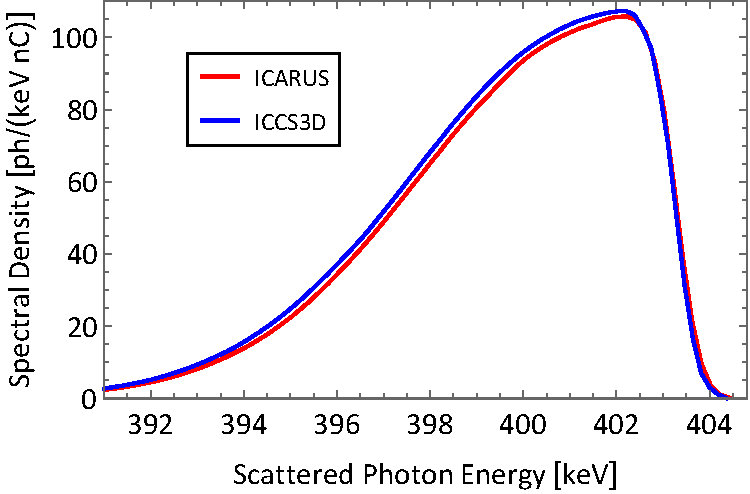
\includegraphics[width=0.8\textwidth]{Figures/CBETA_Inverse_Compton_Source_Design/cbetaspectrumplot_final.pdf}
\caption{Predicted spectral output (flux) from 1064~nm photons colliding head-on with the $E_e =150$~MeV (kinetic energy) electrons in CBETA; this spectrum was generated using the \textsc{ICCS3D} and \textsc{ICARUS} codes. This spectrum has a peak energy of 403.3~keV; using the proposed 5~degree crossing angle, the peak energy is reduced to 402.5~keV and the spectral density is reduced by a factor $\sim$5.}
\label{fig:CBETA_spectrum_benchmarking}
\end{figure}

\section{X-ray ICS Source Comparison}

\begin{table}[!h]
\caption{Comparison of existing and designed x-ray ICS.}
\begin{threeparttable}
\begin{tabular}{lccc}
\hline\hline
ICS & Accelerator Type & Scattered Photon Energy (keV) & Flux (ph/s) \\
\hline
cERL \cite{akagi2016narrow} & ERL & 6.95 & 2.6$\times 10^{7}$ \\ 
ALICE \cite{priebe2008inverse,priebe2010first} & ERL & 21.5 & 9$\times 10^{5}$ \\
MIT ICS\tnote{*} ~\cite{graves2014compact} & Linac & 3 - 30 & 3$\times 10^{14}$ \\
MuCLS \cite{eggl2016munich} & Storage Ring & 15 - 35 & 0.443 - 1.78$\times 10^{10}$ \\ 
Tsinghua \cite{du2013generation} & Linac & 51.7 & 1$\times 10^{6}$ \\
ThomX\tnote{*} ~\cite{variola2014thomx,dupraz2020thomx} & Storage Ring & 45 - 90 & $1\times 10^{10}$ - $10^{13}$ \\
BriXS\tnote{*} ~\cite{faillace2019status,cardarelli2020brixs} & ERL & 20 - 180 & $1\times 10^{10}$ - $10^{13}$ \\
CBETA\tnote{*} & ERL & 32.2, 109.7, 233.1, 402.5 & 3.16 - 3.21$\times 10^{10}$ \\ 
NIJI-IV \cite{sei2017demonstration} & Storage Ring & 1200 & 3.1$\times 10^{4}$ \\ 
HI$\gamma$S\tnote{$\dagger$} ~\cite{weller2009research} & Storage Ring & 1000 - 3000 & 5$\times 10^{7}$ - 5$\times 10^{8}$ \\
\hline\hline
\end{tabular}
\begin{tablenotes}
\item[*]{Denotes design parameters for sources which are not yet demonstrated.}
\item[$\dagger$]{The HI$\gamma$S source is capable of scattered photon energies up to 100~MeV. Shown is the lowest energy operational setting.}
\end{tablenotes}
\end{threeparttable}
\label{tab:xray_ICS_comparison}
\end{table}

\section{Synchrotron Facility Comparison}

\begin{figure}[!h]
\centering
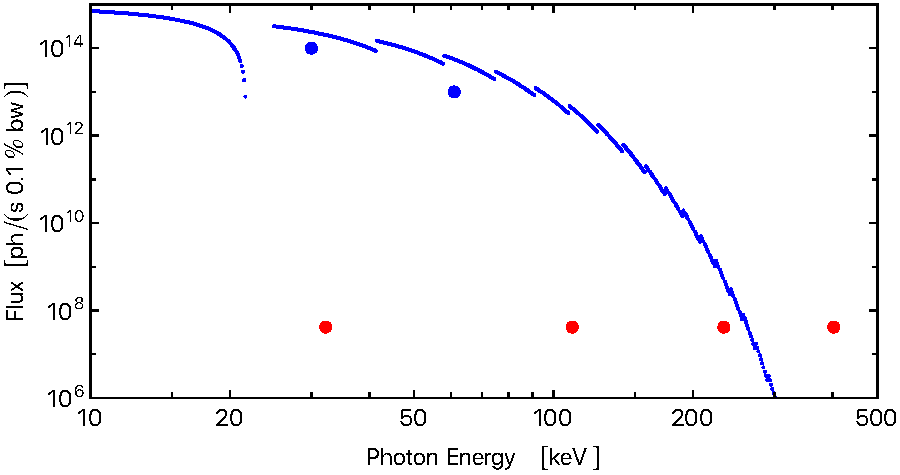
\includegraphics[width=0.8\textwidth]{Figures/CBETA_Inverse_Compton_Source_Design/spring8bl10fluxplot.pdf}
\caption{Comparison of CBETA predicted flux (here flux in a 0.1\% bandwidth to allow comparison with conventional calculations of undulator flux) at the four discrete operating energies given in Table~\ref{tab:CBETA_spectral_output} with the output from a typical high-energy undulator. The undulator shown is the SPRING-8 BL10XU insertion device~\cite{spring8beamlines} assuming an \textit{rms} phase error of 5~degrees. Whilst this undulator is not designed to deliver good output at high harmonic number, it offers a useful guide to possible 3rd-generation source output in the 100~keV to 500~keV range. the measured flux at 30~keV and 61~keV for this beamline is also shown~\cite{spring8beamlines}. We predict that CBETA flux at 402~keV (150~MeV electron energy) exceeds that from 3rd-generation sources.}
\label{fig:ICS_vs_SPRING8_Undulator_Flux}
\end{figure}

\begin{figure}[!h]
\centering
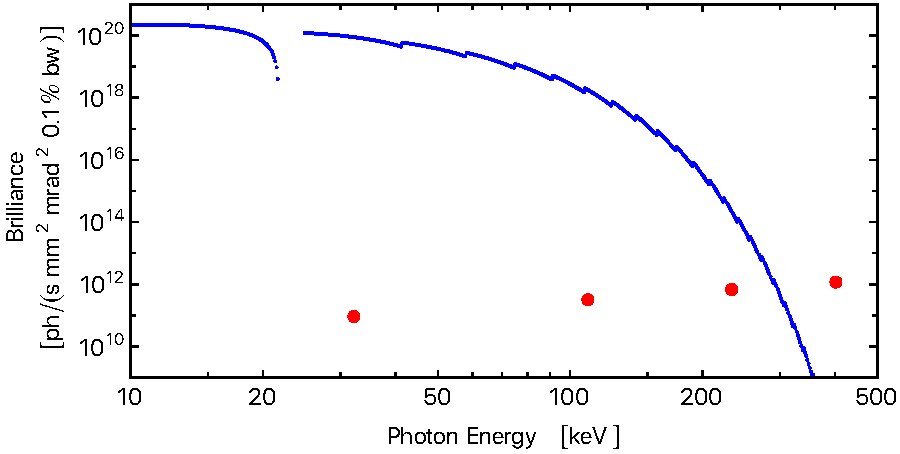
\includegraphics[width=0.8\textwidth]{Figures/CBETA_Inverse_Compton_Source_Design/spring8bl10brillianceplot.pdf}
\caption{Comparison of CBETA predicted brilliance at the four discrete operating energies given in Table~\ref{CBETA_spectral_output} with the output from a typical high-energy undulator. The undulator shown is the SPRING-8 BL10XU insertion device~\cite{spring8beamlines} assuming an \textit{rms} phase error of 5~degrees. We predict that CBETA brilliance at 402~keV (150~MeV electron kinetic energy) exceeds that from 3rd-generation sources.}
\label{fig:ICS_vs_SPRING8_Undulator_Brilliance}
\end{figure}

\begin{figure}[!h]
\centering
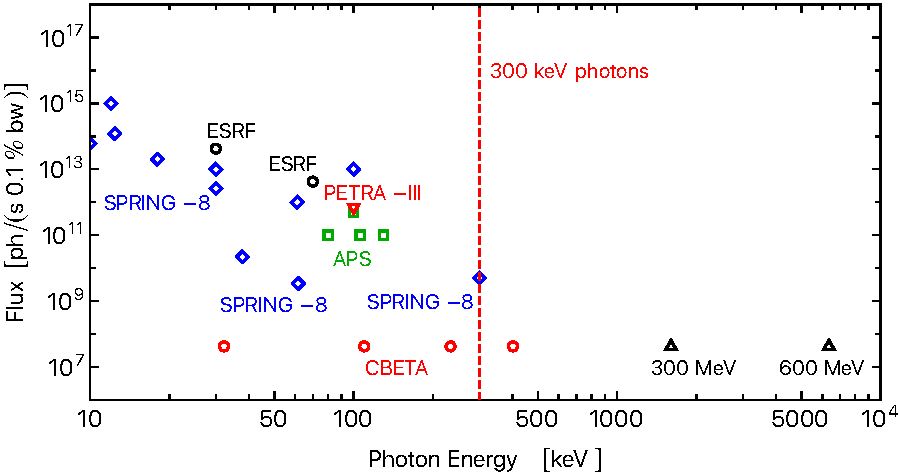
\includegraphics[width=0.8\textwidth]{Figures/CBETA_Inverse_Compton_Source_Design/sourcefluxcomparison.pdf}
\caption{On-sample measured fluxes from APS, ESRF-EBS, PETRA-III, and SPRING-8 for which information has been published~\cite{apsbeamlines,esrfbeamlines,petraiiibeamlines,spring8beamlines}. This is compared with the predicted CBETA outputs in Table~\ref{CBETA_spectral_output}, at the 4 discrete photon energies from 32 to 402~keV, and the predicted flux obtained by scaling the CBETA electron energy to 300~MeV (1600~keV photons) and 600~MeV (6360~keV photons). Whilst 3rd-generation sources are superior to ICS sources up to photon energies around 300~keV, they do not produce useable flux above 400~keV.}
\label{fig:ICS_Undulator_Comparison}
\end{figure}

\end{document}